\documentclass[11pt]{article}
\usepackage{enumerate}
\usepackage{tikz}
\usepackage{fullpage}
\usepackage{fancyhdr}
\usepackage{graphicx}

\usepackage{amsmath, amsfonts, amsthm, amssymb}
\setlength{\parindent}{0pt}
\setlength{\parskip}{5pt plus 1pt}
\pagestyle{empty}

\def\indented#1{\list{}{}\item[]}
\let\indented=\endlist

\newcounter{questionCounter}
\newcounter{partCounter}[questionCounter]
\newenvironment{question}[2][\arabic{questionCounter}]{%
    \setcounter{partCounter}{0}%
    \vspace{.25in} \hrule \vspace{0.5em}%
        \noindent{\bf #2}%
    \vspace{0.8em} \hrule \vspace{.10in}%
    \addtocounter{questionCounter}{1}%
}{}
\renewenvironment{part}[1][\alph{partCounter}]{%
    \addtocounter{partCounter}{1}%
    \vspace{.10in}%
    \begin{indented}%
       {\bf (#1)} %
}{\end{indented}}

%%%%%%%%%%%%%%%%% Identifying Information %%%%%%%%%%%%%%%%%
%% This is here, so that you can make your homework look %%
%% pretty when you compile it.                           %%
%%     DO NOT PUT YOUR NAME ANYWHERE ELSE!!!!            %%
%%%%%%%%%%%%%%%%%%%%%%%%%%%%%%%%%%%%%%%%%%%%%%%%%%%%%%%%%%%
\newcommand{\myname}{Michael Choquette, Rokhini Prabhu}
\newcommand{\myandrew}{mchoquet, rokhinip}
\newcommand{\myhwname}{Assignment 2}
%%%%%%%%%%%%%%%%%%%%%%%%%%%%%%%%%%%%%%%%%%%%%%%%%%%%%%%%%%%

\begin{document}
\thispagestyle{plain}

\begin{center}
{\Large \myhwname} \\
\myname \\
\myandrew \\
\today
\end{center}

\newcommand{\code}[1]{\texttt{#1}}
\begin{question}{Writeup}
We have designed our framework such that in order to implement a dataflow pass,
one would need to provide all of the configurations specified in \texttt{struct
DataflowConfiguration} to the function \texttt{dataflow}.
\begin{enumerate}
\item \texttt{dir} is one of the \texttt{dataflow::FlowDirection} enums that
needs to specify the direction of the analysis
\item \texttt{top} and \texttt{boundaryState} are represented as
\texttt{bitVectors}. As such, the client who is using this interface will need 
to represent their domain as a bitvector and maintain the translation from the 
domain to the bitvector.
\item \texttt{meetFunction} can therefore be specified by one of
\texttt{bvIntersect} or \texttt{bvUnion} which has also be exported in
dataflow.h
\item The \texttt{transferFunctionBuilder} is a class specifies the transfer
function for the flow diagram. We specify 3 different kinds of transfer
functions in this builder. \texttt{makeInstTransferFn} is a transfer function on
a per instruction basis. \texttt{makeInstSeqTransferFn} is a transfer function
on a basic block level. Most often, the latter is just a composition of
\texttt{makeInstTransferFn}s but it is the client's responsibility to make sure
that the transfer functions are composed in the right order, depending on
\texttt{dir}. \\
We also have a third transfer function for phi nodes.
We do not treat phi functions to be part of any basic block and
instead, handle them at the same time as the meet operator. This is because, at
this time, we can specialize the phi instruction with information about the
block's predecessors or successors. This last transfer function is therefore 
\texttt{makePhiSeqTransferFn}.
\end{enumerate}

A reference implementation on how to use this framework can be seen in
\texttt{available.cpp} or \texttt{liveness.cpp}

\end{question}
\begin{question}{Lazy Code Motion}

After the Anticipated expressions pass: Each block is annotated with 
the in and out values of \texttt{anticipated}
\begin{center}
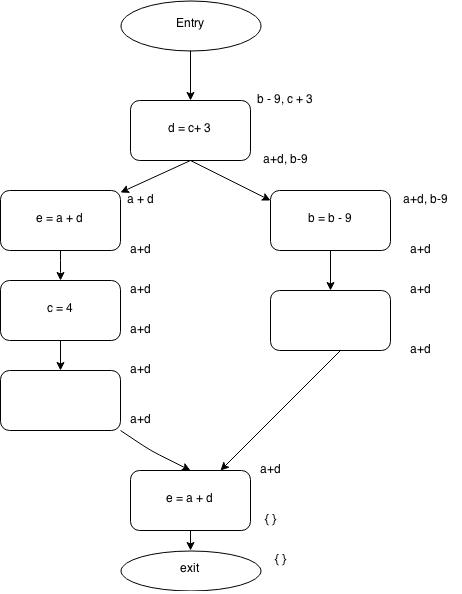
\includegraphics[scale=0.5]{cfg1.jpg}
\end{center}

After the Early Placement pass: Each block is annotated with the values 
of \texttt{earliest} for that block.
\begin{center}
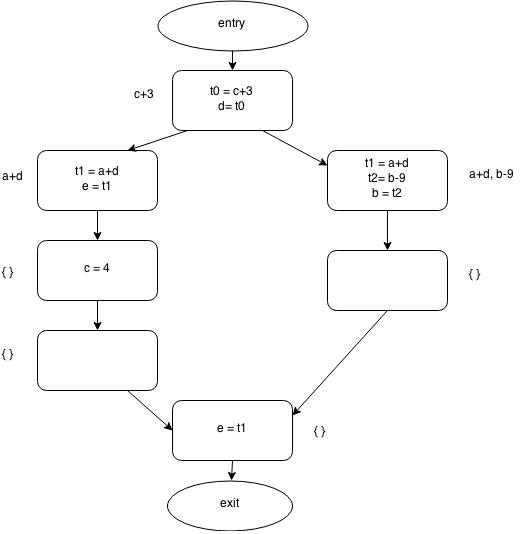
\includegraphics[scale=0.5]{cfg2.jpg}
\end{center}

After Lazy Code Motion and cleanup passes:
\begin{center}
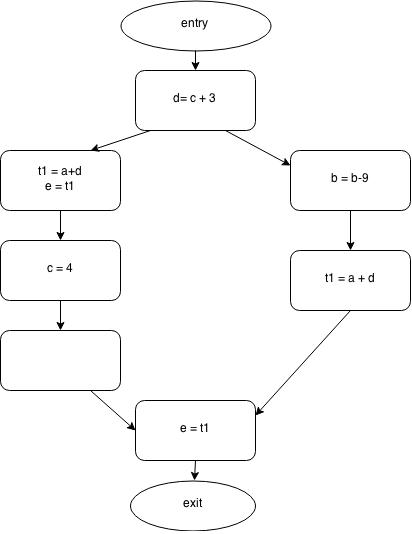
\includegraphics[scale=0.5]{cfg3.jpg}
\end{center}
\end{question}
\newpage
\begin{question}{Loop Invariant Code Motion}
The following lines are loop invariant instructions: $y = 5$, $m = y + 7$, $q =
7$, $r = q + 9$. Since $y=5$ and $q=7$ are assignments to constants inside a
loop, they are clearly loop invariant. $y=5$ is the only definition of $y$ that
is reachable to the statement $m=y+7$ and therefore $m=y+7$ is loop invariant.
The argument for $q$ is identical as well.
\\
\\ We need to satisfy 4 conditions in order to successfully move a statement to
a preheader in the Loop Invariant Code motion Pass. I will now illustrate which
of these statements can be moved and which can't using these requirements. $y=5$ 
cannot be moved since $y$ is assigned to again in the loop. The statements 
$m = y+7$ and $r = q+9$ cannot be moved to a preheader because they are in a 
block that does not dominate all paths to exit. It is possible that the loop 
exits in the very first conditional and therefore never gets around to executing 
the basic block with lines $S9-S12$.
\\
\\The line $q = 7$ can be lifted since it is loop invariant, $q$ is never
redefined, it is in the loop header and therefore, in this case, dominates all
exits of the function as well as all uses of $q$ as well.
\\
\\It is worth noting that with a simple pass of constant propagation and folding, 
we can achieve a much better outcome.
\end{question}
\end{document}
